\section{Kết quả chính từ đợt đo xác nhận mới}

Phần này là trọng tâm thực nghiệm của báo cáo. Khác với các phiên baseline
ban đầu, đợt mới giữ nguyên cohort EC2, lưu route snapshot, đảo thứ tự mode
giữa các block và phân tích trực tiếp raw artifact. Dữ liệu gồm năm block RTT
và ba block ứng dụng, không trộn với dữ liệu pilot.

\subsection{RTT cùng cohort: 5 block và 3.000 probe}

Mỗi block đo ba lượt cho từng mode, mỗi lượt 100 ICMP echo. Toàn bộ
3.000/3.000 probe nhận được phản hồi. Hiệu ứng ghép cặp của block $j$ là

\begin{equation}
\Delta_j=\overline{RTT}_{\mathrm{TGW},j}
-\overline{RTT}_{\mathrm{Peering},j}.
\end{equation}

\begin{figure}[H]
\centering
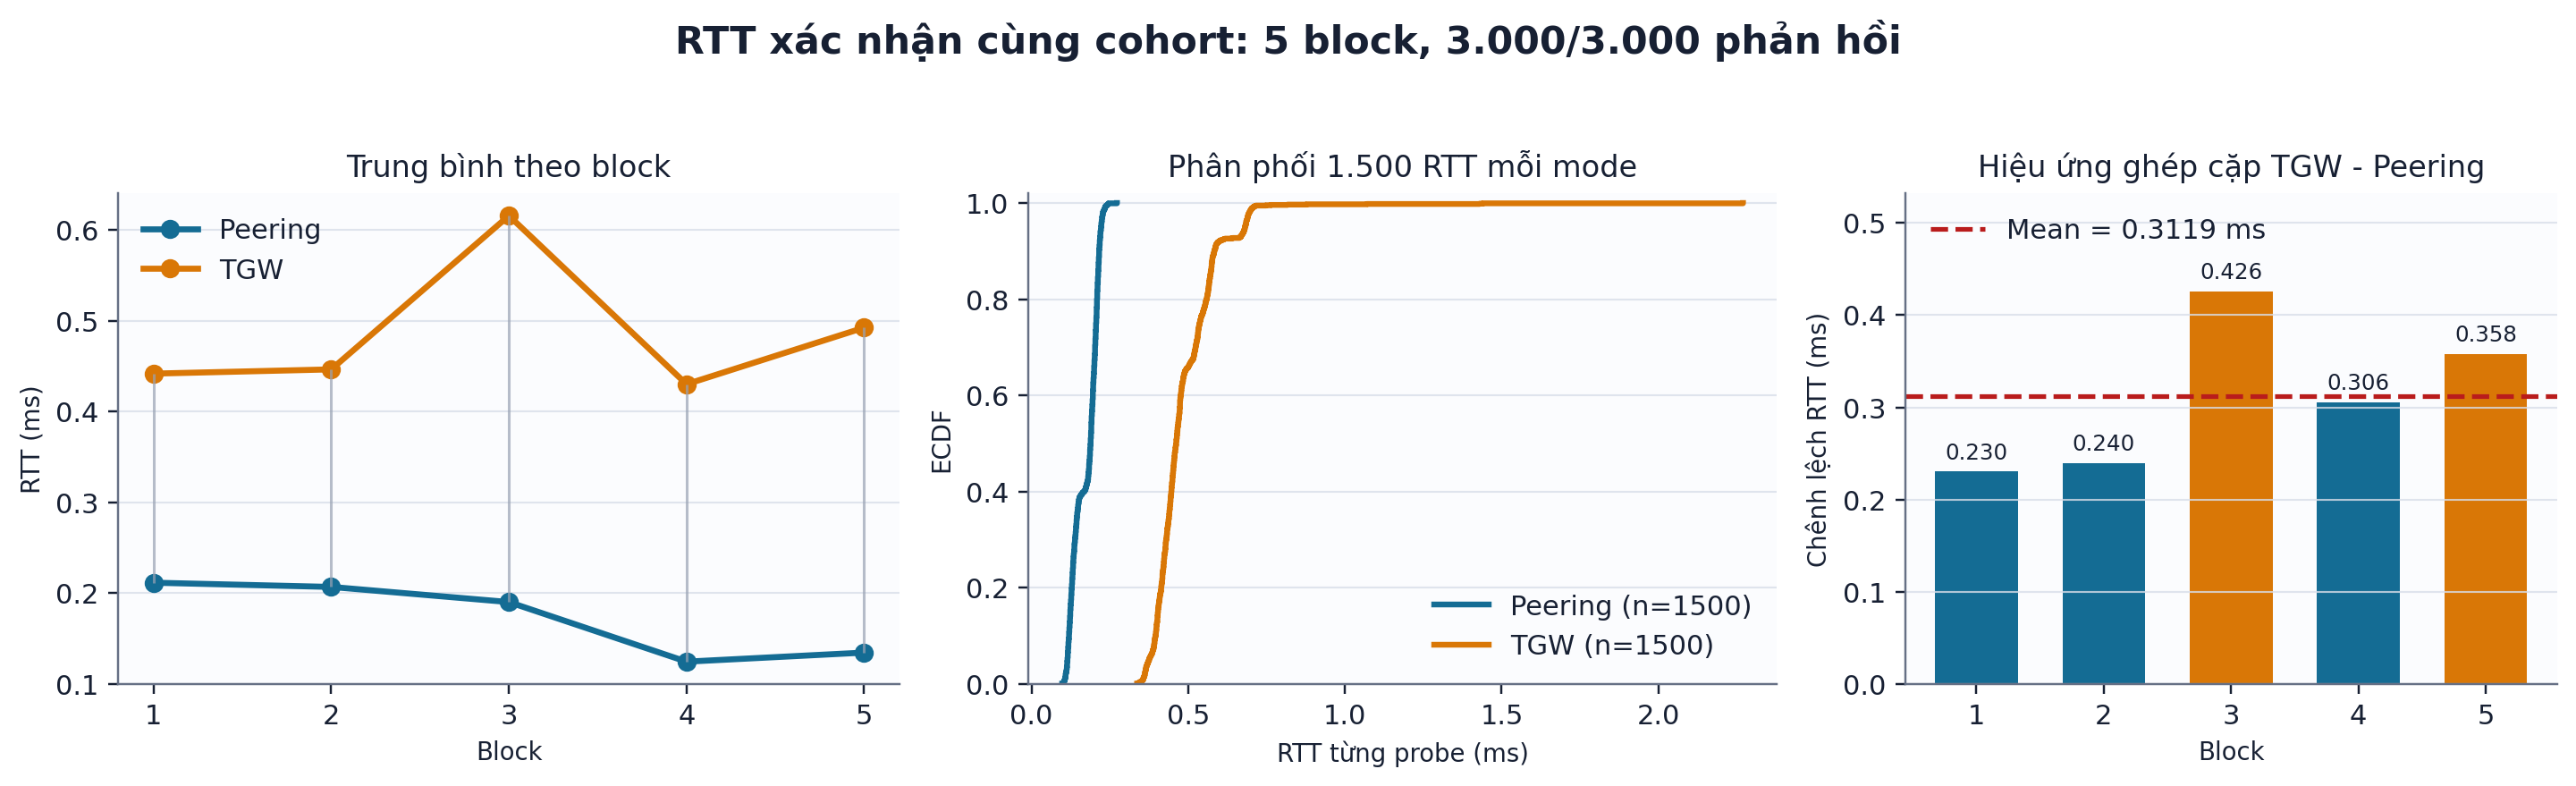
\includegraphics[width=\textwidth]{img/chapter3/primary/rtt-confirmation-dashboard.png}
\caption{Kết quả RTT mới: trung bình block, ECDF của 3.000 probe và hiệu ứng ghép cặp}
\label{fig:rtt-primary}
\end{figure}

\begin{table}[H]
\centering
\caption{RTT trung bình trong năm block xác nhận}
\label{tab:rtt-confirmation}
\begin{tabular}{crrr}
\toprule
\textbf{Block} & \textbf{Peering (ms)} & \textbf{TGW (ms)} & \textbf{$\Delta_j$ (ms)} \\
\midrule
1 & 0,2113 & 0,4417 & 0,2303 \\
2 & 0,2067 & 0,4463 & 0,2397 \\
3 & 0,1900 & 0,6157 & 0,4257 \\
4 & 0,1243 & 0,4300 & 0,3057 \\
5 & 0,1343 & 0,4923 & 0,3580 \\
\midrule
Trung bình & 0,1733 & 0,4852 & 0,3119 \\
Trung vị hiệu ứng & -- & -- & 0,3057 \\
\bottomrule
\end{tabular}
\end{table}

TGW có RTT cao hơn Peering trong cả 5/5 block; hiệu ứng nằm trong khoảng
0,2303--0,4257 ms, trung bình 0,3119 ms. ECDF trong Hình
\ref{fig:rtt-primary} dùng đủ 1.500 probe mỗi mode, cho thấy hai phân phối tách
rõ trong cohort này chứ không chỉ khác nhau ở một giá trị mean. Kết luận này
chỉ áp dụng cho cấu hình đã đo; $\Delta_j$ là chênh lệch end-to-end, không phải
thời gian xử lý nội bộ của TGW.

\subsection{Deadline ứng dụng: 252.000 request}

Ba block hợp lệ bao phủ Peering/TGW, 8/16 slots và 600/800 request/s. Tổng
cộng có 252.000 request theo lịch, tương ứng 504.000 lời gọi worker C/D. Không
điều kiện nào ghi nhận HTTP/JSON fail; request hoàn thành sau 50 ms vẫn bị tính
là không đúng hạn.

\begin{figure}[H]
\centering
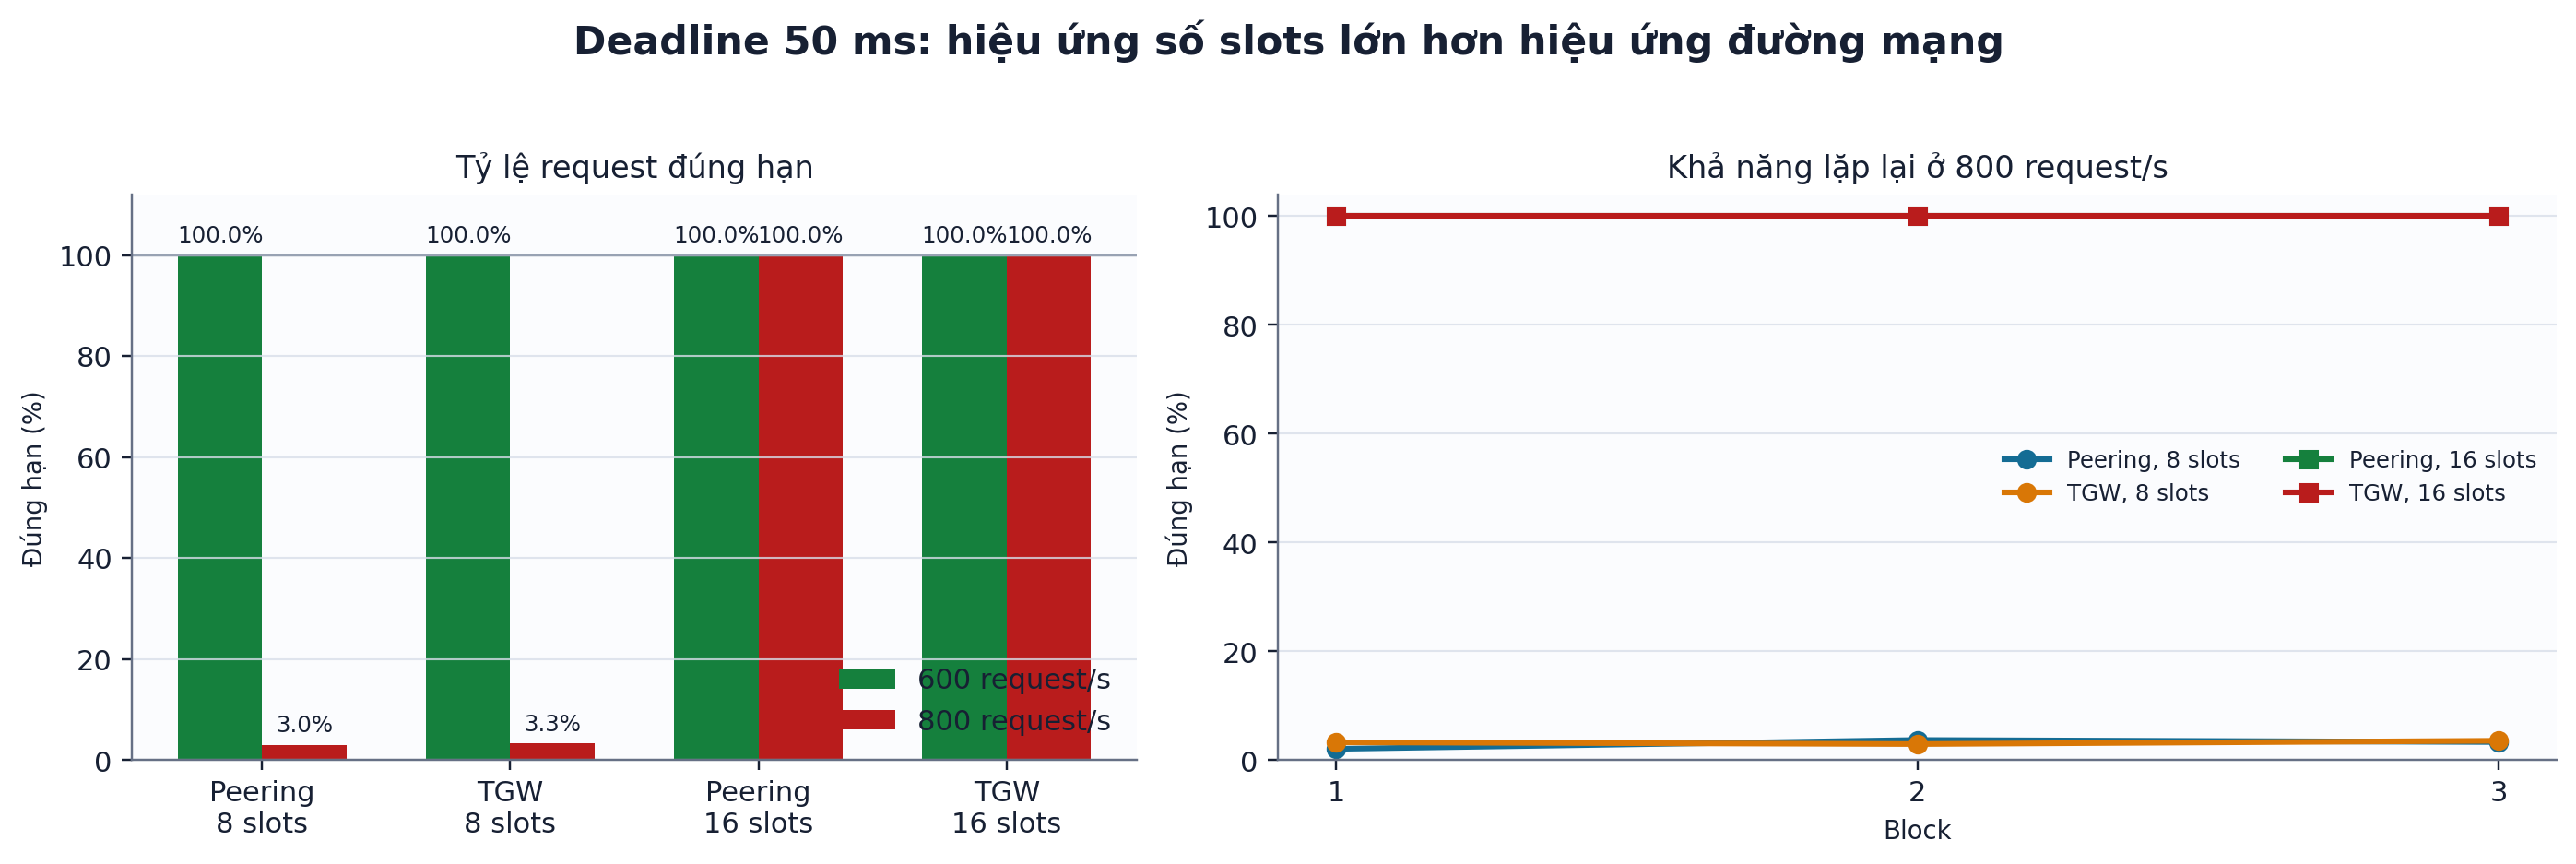
\includegraphics[width=\textwidth]{img/chapter3/primary/application-deadline.png}
\caption{Tỷ lệ đúng hạn và mức lặp lại của hiệu ứng slots trong ba block mới}
\label{fig:deadline-primary}
\end{figure}

Ở 600 request/s, cả tám cấu hình theo mode và slots đều đạt 100\% đúng hạn
trong dữ liệu quan sát. Ở 800 request/s, 8 slots chỉ đạt 1.096/36.000 request
đúng hạn qua Peering và 1.178/36.000 qua TGW, lần lượt 3,0444\% và 3,2722\%.
Khi tăng lên 16 slots, cả hai mode đạt 36.000/36.000 request đúng hạn.

Hiệu ứng $16-8$ slots tại 800 request/s, trung bình qua hai route và ba block,
là 96,8417 điểm phần trăm; từng block nằm trong khoảng
96,5458--97,3167 điểm phần trăm. Vì Peering và TGW đều thất bại với 8 slots và
đều phục hồi với 16 slots, đổi route không giải quyết được giới hạn phục vụ của
worker trong workload này.

\subsection{Cơ chế: tail latency đến từ hàng đợi}

\begin{figure}[H]
\centering
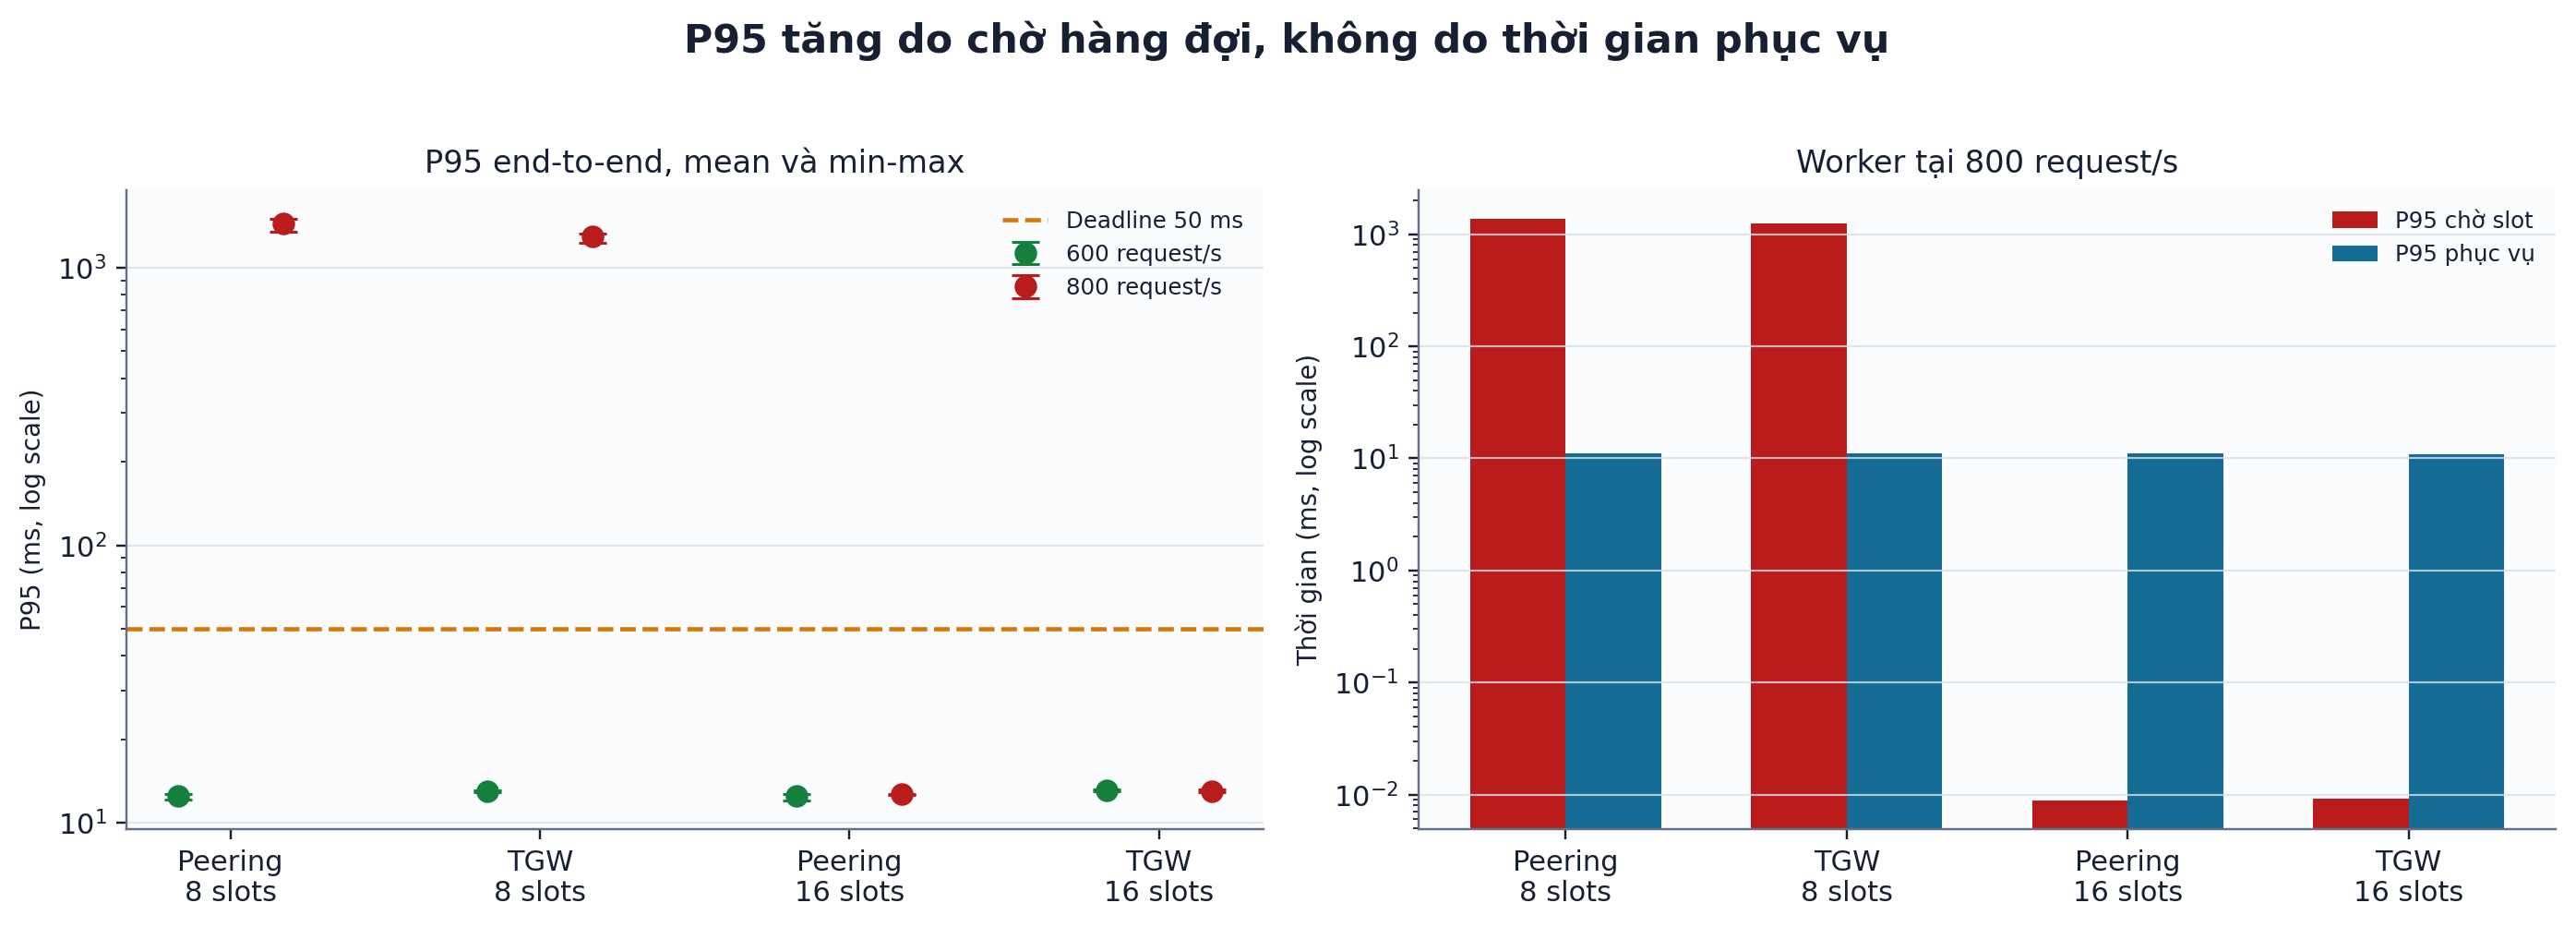
\includegraphics[width=\textwidth]{img/chapter3/primary/application-latency-queue.png}
\caption{P95 end-to-end và phân rã P95 chờ/phục vụ tại worker}
\label{fig:latency-queue-primary}
\end{figure}

Với 800 request/s và 8 slots, P95 end-to-end nằm trong khoảng
1.225,784--1.499,226 ms, vượt xa deadline 50 ms. P95 chờ slot vào khoảng
1,2--1,4 s, trong khi P95 phục vụ vẫn chỉ khoảng 11 ms. Với 16 slots, P95 chờ
giảm xuống dưới 0,013 ms và P95 end-to-end trở lại khoảng 12,651--13,248 ms.
Hình \ref{fig:latency-queue-primary} vì vậy cung cấp chuỗi bằng chứng nhất quán:
tỷ lệ đúng hạn tăng, tail latency giảm, thời gian chờ biến mất, còn thời gian
phục vụ gần như giữ nguyên.

Ví dụ block 3, worker C, Peering, 800 request/s: với 8 slots,
$\lambda_C=732{,}2866$ lời gọi/s và $\overline W_q=0{,}7009511$ s. Định luật
Little trên cohort log hữu hạn cho

\begin{equation}
\overline L_q=\lambda_C\overline W_q
=732{,}2866\times0{,}7009511\approx513{,}2971.
\end{equation}

Với 16 slots ở cùng block/mode/worker, $\lambda_C=799{,}5313$ lời gọi/s,
$\overline W_q=0{,}000005239$ s và $\overline L_q\approx0{,}004189$. Hai giá
trị cho thấy backlog hàng trăm lời gọi đã chuyển thành hàng đợi gần như trống.
Phép tính dùng cùng cửa sổ log và được kiểm tra bằng diện tích occupancy; không
giả định arrival Poisson hay thời gian phục vụ exponential.

\subsection{OpenTelemetry và Grafana}

\begin{figure}[H]
\centering
\begin{subfigure}{0.49\textwidth}
  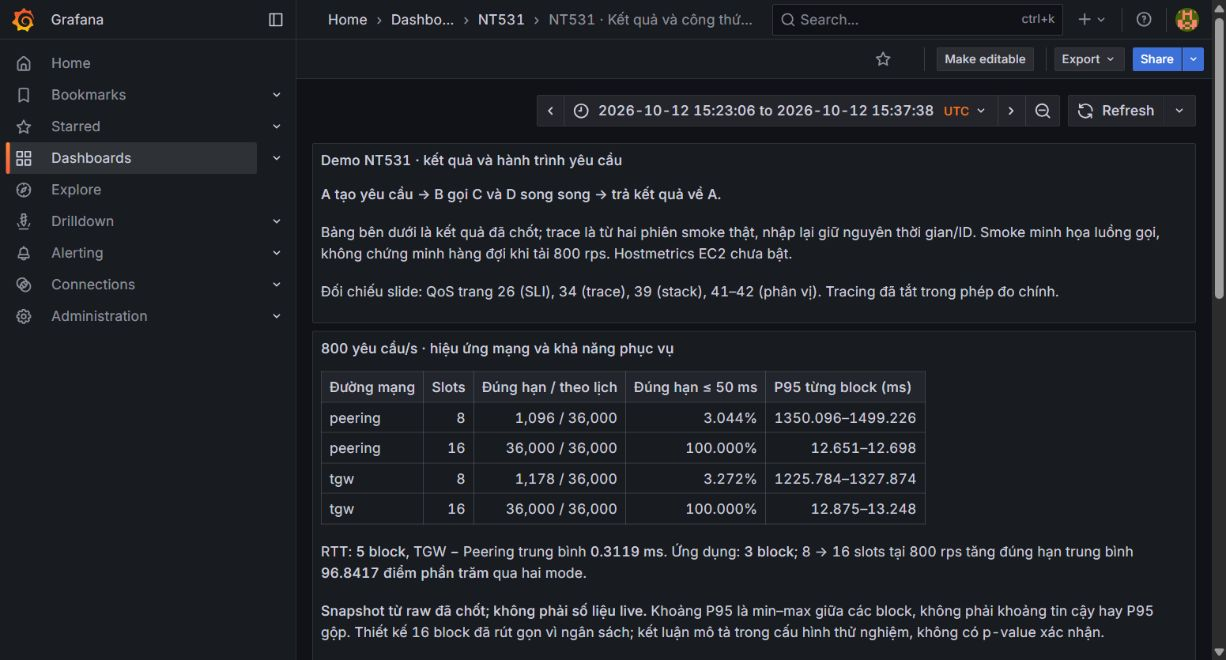
\includegraphics[width=\textwidth]{img/chapter3/observability/grafana-dashboard.jpg}
  \caption{Dashboard tổng hợp}
\end{subfigure}
\hfill
\begin{subfigure}{0.49\textwidth}
  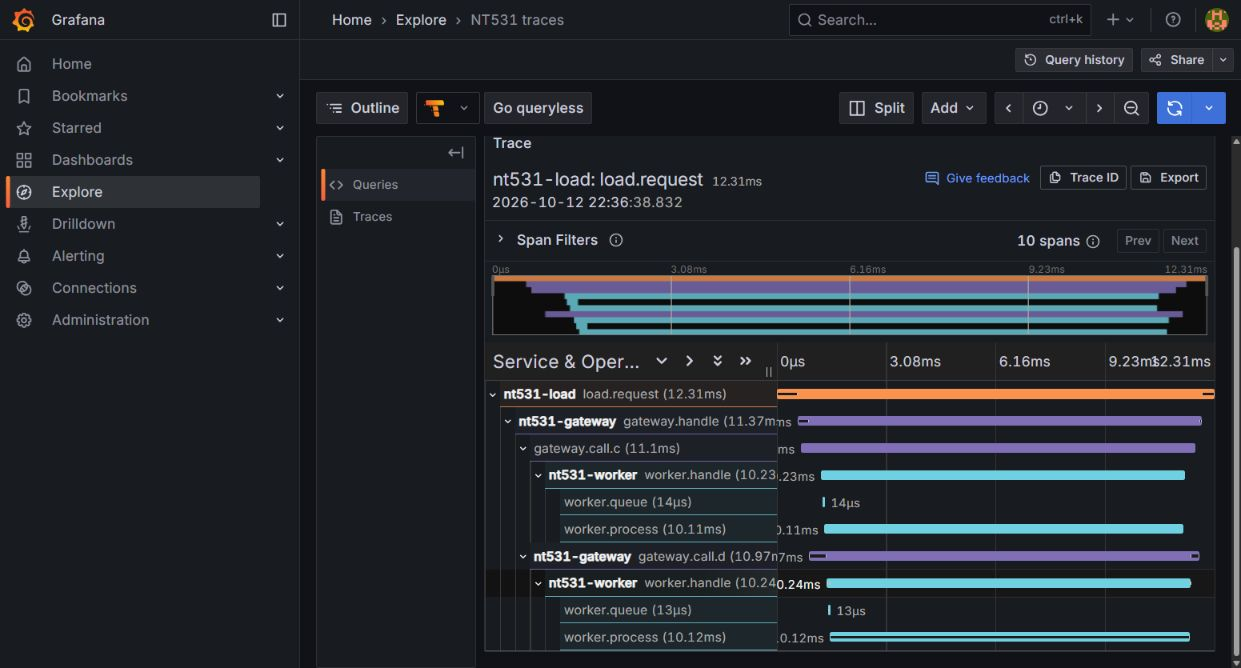
\includegraphics[width=\textwidth]{img/chapter3/observability/trace-waterfall.jpg}
  \caption{Waterfall A--B--C/D}
\end{subfigure}
\caption{Pipeline OpenTelemetry Collector--Tempo--Grafana dùng để giải thích request path}
\label{fig:observability-combined}
\end{figure}

Pipeline đã replay và kiểm tra 12 trace thật, tổng 120 span. Waterfall cho thấy
B gọi C/D song song và cho phép phân biệt queue với service. Trace này là smoke
lịch sử để minh họa cấu trúc request, không phải mẫu benchmark 800 request/s và
không được dùng để tính P95 chính.

\section{Kết luận trực tiếp từ dữ liệu mới}

Ba kết quả mới có mức bằng chứng khác nhau nhưng cùng trả lời một câu hỏi rõ:

\begin{enumerate}
  \item Trong 5/5 block cùng cohort, TGW tăng RTT so với Peering; hiệu ứng ghép
        cặp trung bình là 0,3119 ms.
  \item Tại 800 request/s, đổi Peering/TGW không cứu được cấu hình 8 slots;
        tăng lên 16 slots cải thiện đúng hạn trung bình 96,8417 điểm phần trăm.
  \item P95 phục vụ giữ quanh 11 ms trong khi P95 chờ thay đổi hơn năm bậc độ
        lớn. Hàng đợi ứng dụng là cơ chế chính tạo tail latency trong workload
        này.
\end{enumerate}

Đây là đóng góp mới của đồ án. Kết quả không tuyên bố Peering hoặc TGW thắng
mọi workload; nó chỉ ra khi nào chênh lệch đường mạng đáng chú ý và khi nào
nút thắt ứng dụng lớn đến mức lựa chọn route không còn quyết định SLI.
